\section{初识零件图}
在构建图\ref{fig:xiaoluntaotong}所示零件之前,让我们先来了解一些相关的制图知识。类似于图\ref{fig:xiaoluntaotong}所示的图纸被称为零件图。所谓零件图是用于表达零件的图样,它广泛运用于工程技术设计、施工或产品制造,它是制造、加工、测量、检验的依据,是工程界的共同技术语言,是表达和交流技术思想的必备工具,是工程技术部门的一项重要技术文件。掌握零件图的阅读和绘制不仅是构建零件三维模型的基础,也是从事工程设计和技术的工程技术人员所必须具备的基本能力。一张完整的零件图应包括以下几个组成部分:
\begin{figure}[htbp]
\centering
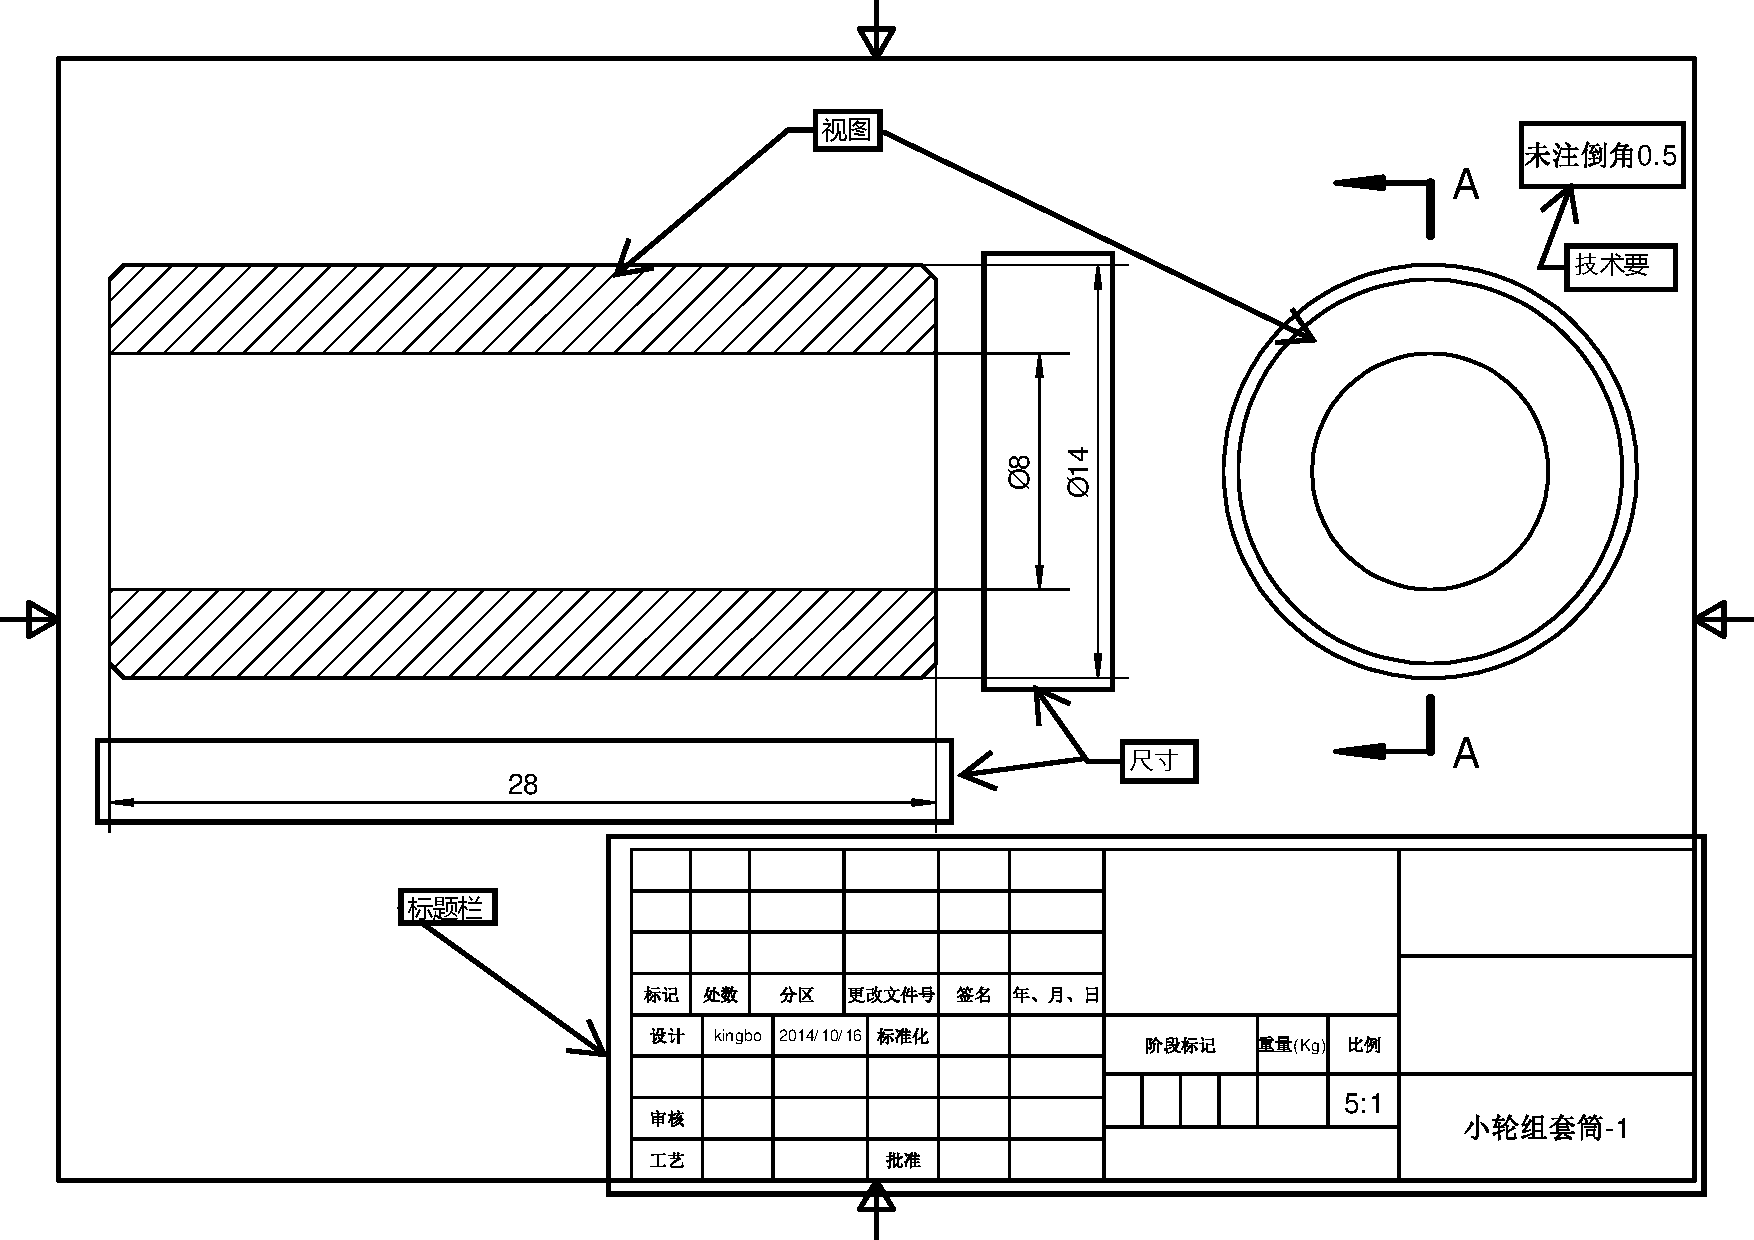
\includegraphics[scale=0.45]{xiaoluntaotong2.pdf}
\caption{零件图组成部分}\label{fig:xiaoluntaotong2}
\end{figure}
图\ref{fig:xiaoluntaotong2}对图\ref{fig:xiaoluntaotong}所示零件图的各个组成部分进行了标注。
\begin{itemize}
\item 一组视图

根据国家制图标准规定的视图、剖视、剖面及其他画法绘制的用于表达零件内外形状的图形。
\item 完整的尺寸

用于确定零件各部分形状大小和位置的全部尺寸。它是按照国家标准GT/T4458.4-1984的要求进行标注的。
\item 技术要求

用于规定零件在制造和检验时应达到的一些要求。通常用规定的符号标注于图纸中或在图纸上指定位置用文字统一标出。
\item 标题栏

用于说明零件的名称、材料、数量等信息。它是按照国家标准GB/T10609.1-1989的规定绘制的。
\end{itemize}

\section{圆柱体视图}
图\ref{fig:xiaoluntaotong}所示零件图中的视图既然是用于表达零件的内外形状的,那么它的立体形状是怎样的呢,如保用AutoCAD构建出它的三维模型呢?要解决这个问题,我们先将图\ref{fig:xiaoluntaotong}所示零件图进行简化,忽略其内部及细微的局部,只研究其中$\phi 14$所对应的部分,简化后的结果如图\ref{fig:yuanzhuti}所示。
\begin{figure}[htbp]
\centering
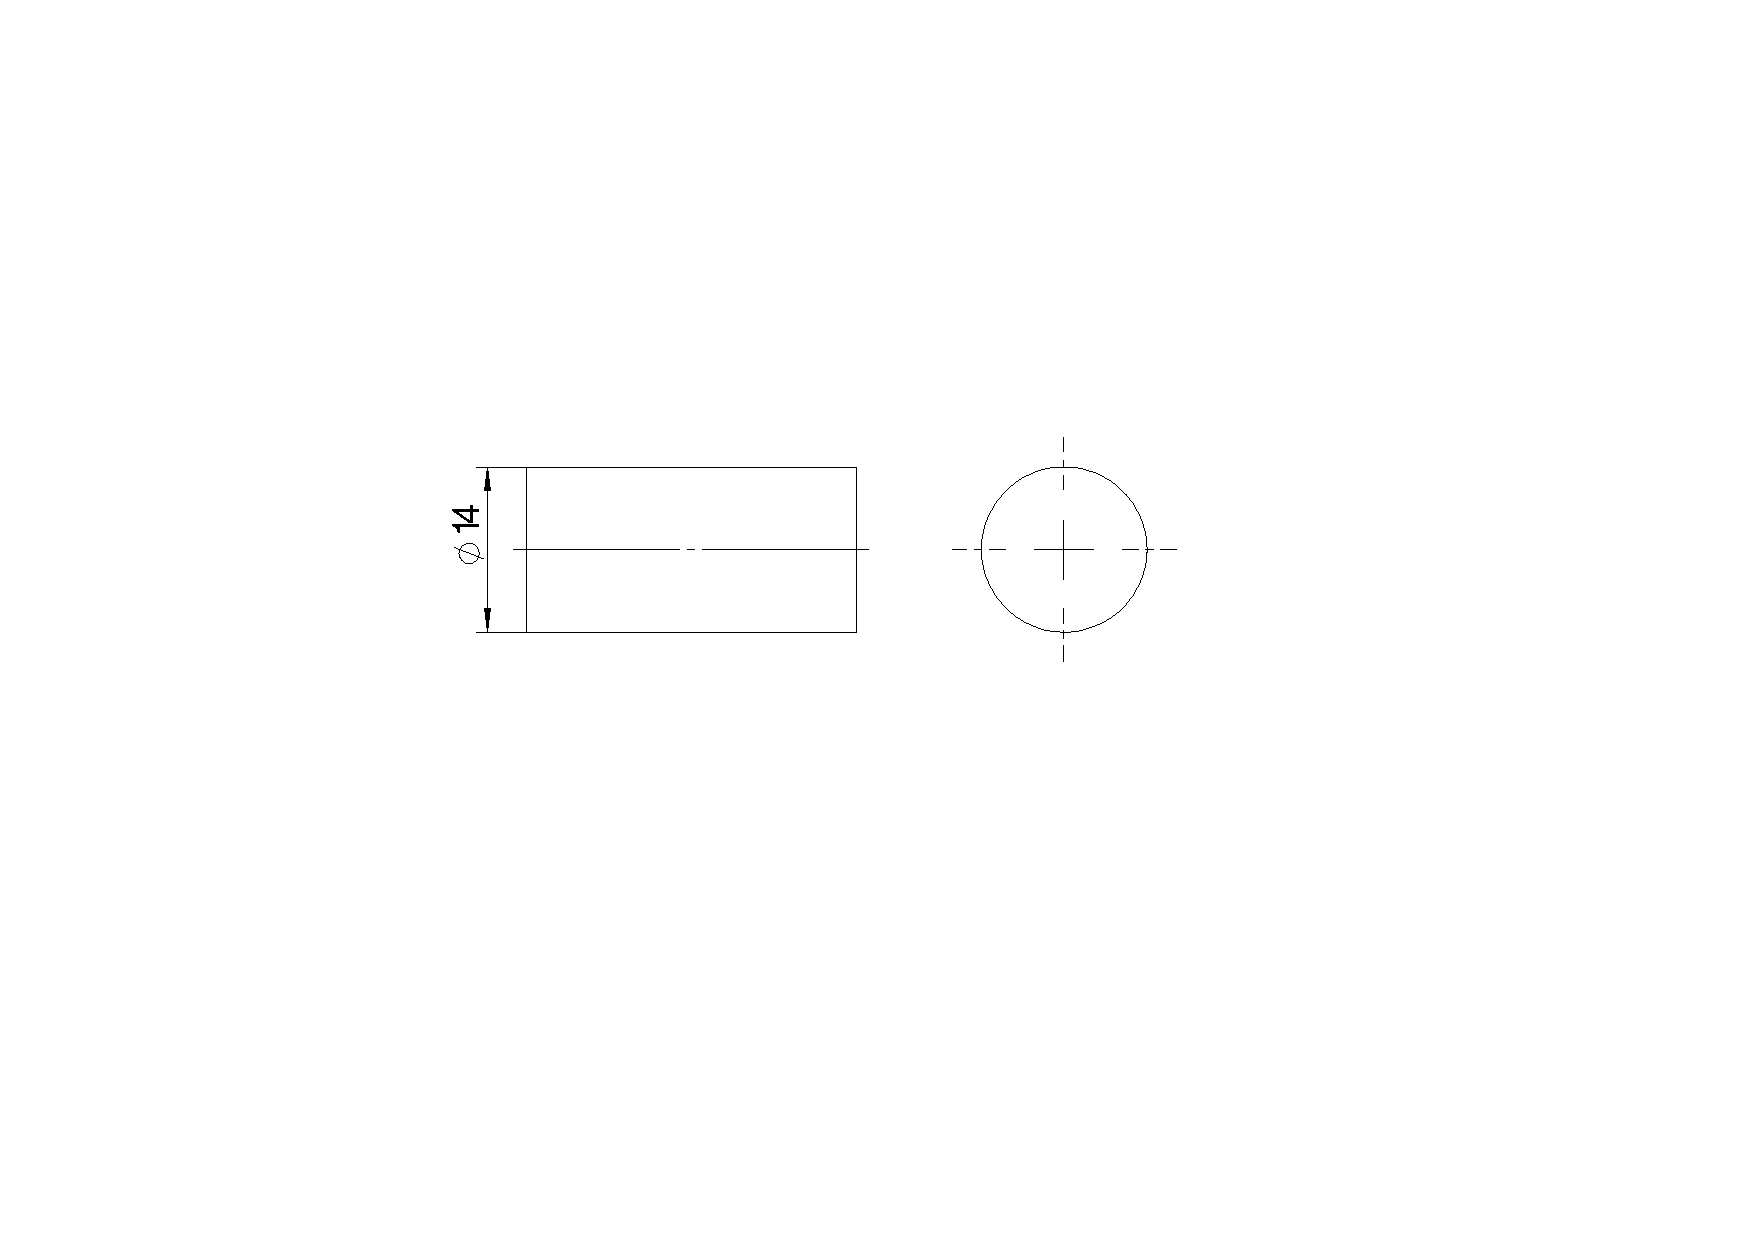
\includegraphics[scale=0.55]{yuanzhuti.pdf}
\caption{套筒外圆柱视图}\label{fig:yuanzhuti}
\end{figure}

那么图\ref{fig:yuanzhuti}所表达的又是什么物体呢?要回答这个问题,我们先将一个圆柱体放置于图\ref{fig:sanweizuobiao}所示的三个相互垂直的三面投影之中,然后从三个方向将圆柱体投影到投影面上,即可得到圆柱体的三面投影,如图\ref{fig:yuanzhutouyin}所示。从圆柱体的三面投影可以看出其中两投影的大小和形状是一样的,均为矩形,仅有一个投影为圆。
\begin{figure}[htbp]
\centering
\subfloat[三维投影面]{\label{fig:sanweizuobiao}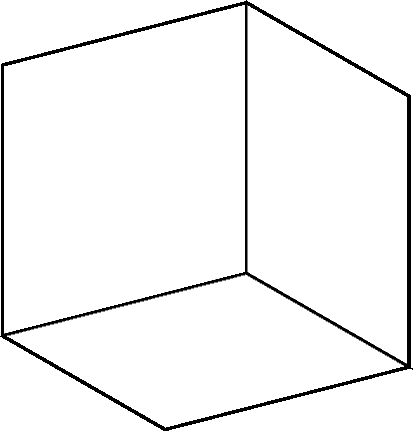
\includegraphics[scale=0.4]{sanweizuobiao.png}}\hspace{30pt}
\subfloat[圆柱体三面投影]{\label{fig:yuanzhutouyin}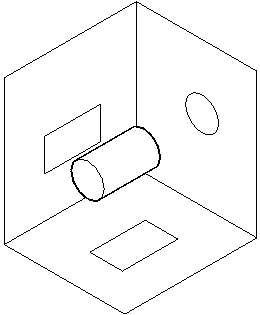
\includegraphics[scale=0.3]{yuanzhutouyin.png}}
\end{figure}

由此可以看出图\ref{fig:yuanzhuti}所示的视图表达的是一个直径为$\phi 14$,长为28的圆柱体,其中符号$\phi$用于表示后面所标注的尺寸是直径。

\yaodian{合理的忽略细节是简化和加速模型构建的关键。}
\endinput